\documentclass[]{article}
\usepackage{lmodern}
\usepackage{amssymb,amsmath}
\usepackage{ifxetex,ifluatex}
\usepackage{fixltx2e} % provides \textsubscript
\ifnum 0\ifxetex 1\fi\ifluatex 1\fi=0 % if pdftex
  \usepackage[T1]{fontenc}
  \usepackage[utf8]{inputenc}
\else % if luatex or xelatex
  \ifxetex
    \usepackage{mathspec}
  \else
    \usepackage{fontspec}
  \fi
  \defaultfontfeatures{Ligatures=TeX,Scale=MatchLowercase}
\fi
% use upquote if available, for straight quotes in verbatim environments
\IfFileExists{upquote.sty}{\usepackage{upquote}}{}
% use microtype if available
\IfFileExists{microtype.sty}{%
\usepackage{microtype}
\UseMicrotypeSet[protrusion]{basicmath} % disable protrusion for tt fonts
}{}
\usepackage[margin=1in]{geometry}
\usepackage{hyperref}
\hypersetup{unicode=true,
            pdftitle={R: Transformación de datos},
            pdfborder={0 0 0},
            breaklinks=true}
\urlstyle{same}  % don't use monospace font for urls
\usepackage{color}
\usepackage{fancyvrb}
\newcommand{\VerbBar}{|}
\newcommand{\VERB}{\Verb[commandchars=\\\{\}]}
\DefineVerbatimEnvironment{Highlighting}{Verbatim}{commandchars=\\\{\}}
% Add ',fontsize=\small' for more characters per line
\usepackage{framed}
\definecolor{shadecolor}{RGB}{248,248,248}
\newenvironment{Shaded}{\begin{snugshade}}{\end{snugshade}}
\newcommand{\KeywordTok}[1]{\textcolor[rgb]{0.13,0.29,0.53}{\textbf{#1}}}
\newcommand{\DataTypeTok}[1]{\textcolor[rgb]{0.13,0.29,0.53}{#1}}
\newcommand{\DecValTok}[1]{\textcolor[rgb]{0.00,0.00,0.81}{#1}}
\newcommand{\BaseNTok}[1]{\textcolor[rgb]{0.00,0.00,0.81}{#1}}
\newcommand{\FloatTok}[1]{\textcolor[rgb]{0.00,0.00,0.81}{#1}}
\newcommand{\ConstantTok}[1]{\textcolor[rgb]{0.00,0.00,0.00}{#1}}
\newcommand{\CharTok}[1]{\textcolor[rgb]{0.31,0.60,0.02}{#1}}
\newcommand{\SpecialCharTok}[1]{\textcolor[rgb]{0.00,0.00,0.00}{#1}}
\newcommand{\StringTok}[1]{\textcolor[rgb]{0.31,0.60,0.02}{#1}}
\newcommand{\VerbatimStringTok}[1]{\textcolor[rgb]{0.31,0.60,0.02}{#1}}
\newcommand{\SpecialStringTok}[1]{\textcolor[rgb]{0.31,0.60,0.02}{#1}}
\newcommand{\ImportTok}[1]{#1}
\newcommand{\CommentTok}[1]{\textcolor[rgb]{0.56,0.35,0.01}{\textit{#1}}}
\newcommand{\DocumentationTok}[1]{\textcolor[rgb]{0.56,0.35,0.01}{\textbf{\textit{#1}}}}
\newcommand{\AnnotationTok}[1]{\textcolor[rgb]{0.56,0.35,0.01}{\textbf{\textit{#1}}}}
\newcommand{\CommentVarTok}[1]{\textcolor[rgb]{0.56,0.35,0.01}{\textbf{\textit{#1}}}}
\newcommand{\OtherTok}[1]{\textcolor[rgb]{0.56,0.35,0.01}{#1}}
\newcommand{\FunctionTok}[1]{\textcolor[rgb]{0.00,0.00,0.00}{#1}}
\newcommand{\VariableTok}[1]{\textcolor[rgb]{0.00,0.00,0.00}{#1}}
\newcommand{\ControlFlowTok}[1]{\textcolor[rgb]{0.13,0.29,0.53}{\textbf{#1}}}
\newcommand{\OperatorTok}[1]{\textcolor[rgb]{0.81,0.36,0.00}{\textbf{#1}}}
\newcommand{\BuiltInTok}[1]{#1}
\newcommand{\ExtensionTok}[1]{#1}
\newcommand{\PreprocessorTok}[1]{\textcolor[rgb]{0.56,0.35,0.01}{\textit{#1}}}
\newcommand{\AttributeTok}[1]{\textcolor[rgb]{0.77,0.63,0.00}{#1}}
\newcommand{\RegionMarkerTok}[1]{#1}
\newcommand{\InformationTok}[1]{\textcolor[rgb]{0.56,0.35,0.01}{\textbf{\textit{#1}}}}
\newcommand{\WarningTok}[1]{\textcolor[rgb]{0.56,0.35,0.01}{\textbf{\textit{#1}}}}
\newcommand{\AlertTok}[1]{\textcolor[rgb]{0.94,0.16,0.16}{#1}}
\newcommand{\ErrorTok}[1]{\textcolor[rgb]{0.64,0.00,0.00}{\textbf{#1}}}
\newcommand{\NormalTok}[1]{#1}
\usepackage{graphicx,grffile}
\makeatletter
\def\maxwidth{\ifdim\Gin@nat@width>\linewidth\linewidth\else\Gin@nat@width\fi}
\def\maxheight{\ifdim\Gin@nat@height>\textheight\textheight\else\Gin@nat@height\fi}
\makeatother
% Scale images if necessary, so that they will not overflow the page
% margins by default, and it is still possible to overwrite the defaults
% using explicit options in \includegraphics[width, height, ...]{}
\setkeys{Gin}{width=\maxwidth,height=\maxheight,keepaspectratio}
\IfFileExists{parskip.sty}{%
\usepackage{parskip}
}{% else
\setlength{\parindent}{0pt}
\setlength{\parskip}{6pt plus 2pt minus 1pt}
}
\setlength{\emergencystretch}{3em}  % prevent overfull lines
\providecommand{\tightlist}{%
  \setlength{\itemsep}{0pt}\setlength{\parskip}{0pt}}
\setcounter{secnumdepth}{0}
% Redefines (sub)paragraphs to behave more like sections
\ifx\paragraph\undefined\else
\let\oldparagraph\paragraph
\renewcommand{\paragraph}[1]{\oldparagraph{#1}\mbox{}}
\fi
\ifx\subparagraph\undefined\else
\let\oldsubparagraph\subparagraph
\renewcommand{\subparagraph}[1]{\oldsubparagraph{#1}\mbox{}}
\fi

%%% Use protect on footnotes to avoid problems with footnotes in titles
\let\rmarkdownfootnote\footnote%
\def\footnote{\protect\rmarkdownfootnote}

%%% Change title format to be more compact
\usepackage{titling}

% Create subtitle command for use in maketitle
\newcommand{\subtitle}[1]{
  \posttitle{
    \begin{center}\large#1\end{center}
    }
}

\setlength{\droptitle}{-2em}
  \title{R: Transformación de datos}
  \pretitle{\vspace{\droptitle}\centering\huge}
  \posttitle{\par}
  \author{}
  \preauthor{}\postauthor{}
  \date{}
  \predate{}\postdate{}

\usepackage[
  backend=biber,
  style=alphabetic,
  sorting=ynt,
  citestyle=authoryear
  ]{biblatex}
\addbibresource{../lit/bib.bib}

\usepackage[utf8]{inputenc}
\usepackage[spanish]{babel}

\usepackage{float}
\usepackage{enumitem}
\newcommand\novspace{\@minipagetrue}

%%%% Frames
\ifxetex
    \makeatletter % undo the wrong changes made by mathspec
    \let\RequirePackage\original@RequirePackage
    \let\usepackage\RequirePackage
    \makeatother
\fi

\usepackage{xcolor}
\usepackage[tikz]{bclogo}
\usepackage[framemethod=tikz]{mdframed}
\usepackage{lipsum}
\usepackage[many]{tcolorbox}

\definecolor{bgblue}{RGB}{245,243,253}
\definecolor{ttblue}{RGB}{91,194,224}
\definecolor{llred}{RGB}{255,228,225}
\definecolor{bbblack}{RGB}{0,0,0}

\mdfdefinestyle{mystyle}{%
  rightline=true,
  innerleftmargin=10,
  innerrightmargin=10,
  outerlinewidth=3pt,
  topline=false,
  rightline=true,
  bottomline=false,
  skipabove=\topsep,
  skipbelow=\topsep
}

\newtcolorbox{curiosidad}[1][]{
  breakable,
  title=#1,
  colback=white,
  colbacktitle=white,
  coltitle=black,
  fonttitle=\bfseries,
  bottomrule=0pt,
  toprule=0pt,
  leftrule=3pt,
  rightrule=3pt,
  titlerule=0pt,
  arc=0pt,
  outer arc=0pt,
  colframe=black,
}

\newtcolorbox{nota}[1][]{
  breakable,
  freelance,
  title=#1,
  colback=white,
  colbacktitle=white,
  coltitle=black,
  fonttitle=\bfseries,
  bottomrule=0pt,
  boxrule=0pt,
  colframe=white,
  overlay unbroken and first={
  \draw[red!75!black,line width=3pt]
    ([xshift=5pt]frame.north west) -- 
    (frame.north west) -- 
    (frame.south west);
  \draw[red!75!black,line width=3pt]
    ([xshift=-5pt]frame.north east) -- 
    (frame.north east) -- 
    (frame.south east);
  },
  overlay unbroken app={
  \draw[red!75!black,line width=3pt,line cap=rect]
    (frame.south west) -- 
    ([xshift=5pt]frame.south west);
  \draw[red!75!black,line width=3pt,line cap=rect]
    (frame.south east) -- 
    ([xshift=-5pt]frame.south east);
  },
  overlay middle and last={
  \draw[red!75!black,line width=3pt]
    (frame.north west) -- 
    (frame.south west);
  \draw[red!75!black,line width=3pt]
    (frame.north east) -- 
    (frame.south east);
  },
  overlay last app={
  \draw[red!75!black,line width=3pt,line cap=rect]
    (frame.south west) --
    ([xshift=5pt]frame.south west);
  \draw[red!75!black,line width=3pt,line cap=rect]
    (frame.south east) --
    ([xshift=-5pt]frame.south east);
  },
}

\begin{document}


\section{Transformación de datos}\label{transformacion-de-datos}

Esta sección resume algunas de las funciones existentes para
\textbf{transformar} datos en \texttt{R}. En particular, se revisan las
transformaciones más comunes que se realizan sobre datos. En esta
sección, se revisan las acciones implementadas en el paquete
\texttt{dplyr} \parencite{dplyr}. En la figura \ref{fig:ciclo3} podemos
ver la etapa del análisis de datos correspondiente.

\begin{figure}[h]
    \centering
    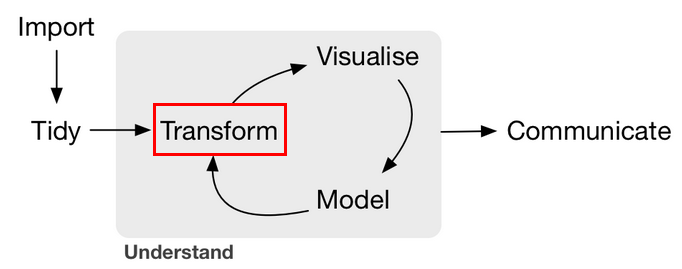
\includegraphics[width=0.75\textwidth]{../img/02_ciclo_3.png}
    \caption{Transformación de datos \textcite[Introducción]{grolemund2016r}.}
    \label{fig:ciclo3}
\end{figure}

Existen muchas maneras de transformar los datos y una gran cantidad de
paquetes que implementan distintas funciones útiles para realizar esta
tarea. En particular, resaltamos \texttt{dplyr} y \texttt{data.table}.
En esta sección se ejemplifican todas las funciones que permiten hacer
trabajo con datos que están implementadas en
\texttt{dplyr}\footnote{Para iniciar en \texttt{data.table} se recomienda ver \textcite{datatabletutorial} así como las viñetas del paquete \textcite{datatable}.}
y en \texttt{tidyr} \parencite{tidyr}.

\subsection{Tareas comunes en la manipulación de
datos}\label{tareas-comunes-en-la-manipulacion-de-datos}

Las funciones implementadas en este paquete están diseñadas para
facilitar la transformación de datos. En general, la transformación de
datos implica definir qué se hará con ellos, escribir un programa que
realice esa tarea y ejecutarlo
\parencite[][viñeta de introducción]{dplyr}.

\texttt{dplyr} y \texttt{tidyr} simplifican estos pasos al proveer de
opciones limitadas consideradas como las tareas más comunes en la
transformación de datos. Además, proveen de verbos simples que
corresponden a funciones en \texttt{R} y que mapean directamente a estas
\emph{tareas más comunes} (ver Tabla \ref{tab:accionescomunes}).

\begin{table}[H]
\centering
\scriptsize{
\begin{tabular}{p{4cm}p{10cm}}
  \hline
Acción & Verbos \\ 
\hline
Extracción de \textbf{subconjuntos de observaciones}. & 
  \parbox[t]{10cm}{
    \begin{itemize} 
      \item{\texttt{filter}: seleccionamos filas de acuerdo a los valores de las variables} 
      \item{\texttt{distinct}: elimina renglones duplicados}
      \item{\texttt{sample\_frac}: selecciona aleatoriamente una fracción de filas}
      \item{\texttt{sample\_n}: selecciona aleatoriamente $n$ filas}
      \item{\texttt{slice}: selecciona filas por posición}
      \item{\texttt{top\_n}: selecciona y ordena según una variable $n$ entradas\\}
    \end{itemize} 
  } \\
\hline
Extracción de \textbf{subconjuntos de variables}. &  
  \parbox[t]{10cm}{
    \begin{itemize} 
      \item{\texttt{select}: seleccionamos un subconjunto de las columnas utilizando los nombres de las variables\\}
    \end{itemize} 
  } \\
\hline
Creación de \textbf{resumenes de datos}. & 
  \parbox[t]{10cm}{
    \begin{itemize} 
      \item{\texttt{summarise}: resume los datos en un valor único}
      \item{\texttt{summarise\_each}: aplica una función de resumen a cada columna}
      \item{\texttt{count}: cuenta el número de filas con cada valor única de una variable\\}
    \end{itemize} 
  } \\
\hline
Creación de \textbf{nuevas variables}. &
  \parbox[t]{10cm}{
    \begin{itemize} 
      \item{\texttt{mutate}: genera nuevas variables a partir de las variables originales}
      \item{\texttt{mutate\_each}: aplica una función ventana a cada columna}
      \item{\texttt{transmute}: genera una o más nuevas columnas eliminando las columnas originales\\}
    \end{itemize} 
  } \\
\hline
\textbf{Combinación} de conjuntos de datos. & 
  \parbox[t]{10cm}{
    \begin{itemize} 
      \item{\texttt{left\_join}: realiza un join conservando todas las observaciones de la primera tabla especificada}
      \item{\texttt{right\_join}: realiza un join conservando todas las observaciones de la segunda tabla especificada}
      \item{\texttt{inner\_join}: realiza un join conservando todas las observaciones que están en ambas tablas}
      \item{\texttt{full\_join}: realiza un join conservando todas las observaciones y valores de ambas tablas}
      \item{\texttt{semi\_join}: conserva todas las observaciones de la primera tabla que están en la segunda tabla}
      \item{\texttt{anti\_join}: conserva todas las observaciones de la primera tabla que no están en la segunda tabla}
      \item{\texttt{intersect}: conserva observaciones que están tanto en la primera tabla como en la segunda}
      \item{\texttt{union}: conserva observaciones que están en cualesquier tabla}
      \item{\texttt{setdiff}: conserva observaciones de la primera tabla que no están en la segunda}
      \item{\texttt{bind\_rows}: une las filas de la segunda tabla a las de la primera}
      \item{\texttt{bind\_cols}: une las columnas de la segunda tabla a las de la primera\\}
    \end{itemize} 
  } \\
\hline
\textbf{Agrupar} datos. & 
  \parbox[t]{10cm}{
    \begin{itemize} 
      \item{\texttt{group\_by}: agrupa los datos según una o más variables}
      \item{\texttt{ungroup}: elimina los grupos en un data frame\\}
    \end{itemize} 
  } \\
\hline
\textbf{Reorganizar} datos (\textit{reshape data}). & 
  \parbox[t]{10cm}{
    \begin{itemize} 
      \item{\texttt{data\_frame}: combina vectores en un dataframe}
      \item{\texttt{arrange}: Ordena las filas según una o más variables}
      \item{\texttt{rename}: renombra columnas de un dataframe\\}
    \end{itemize} 
  } \\
\hline
\end{tabular}
}
\caption{Acciones y verbos comunes en la manipulación de datos \parencite{datawrangling}.} 
\label{tab:accionescomunes}
\end{table}

Dentro de \texttt{tidyr} hay más verbos útiles para reorganizar datos
que se verán en la sección \ref{datos-limpios} junto con los
\emph{criterios de datos limpios} que proporcionan un sustento para la
conceptualización de la manipulación de datos eficiente en \texttt{R}.

Todos estos verbos funcionan de la misma manera (tienen la misma
estructura):

\begin{itemize}
\tightlist
\item
  El primer argumento de la función es un \emph{data.frame}
\item
  Los argumentos subsecuentes indican qué es lo que se debe hacer a ese
  \emph{data.frame}
\item
  Siempre regresa un \emph{data.frame}
\end{itemize}

A continuación, se ejemplifica el uso de los distintos verbos de la
tabla \ref{tab:accionescomunes}. Para esto, utilizaremos los siguientes
conjuntos de datos de muestra, todos disponibles en el paquete
\texttt{nycflights13} \parencite{flights}. Se leerán desde archivo de
texto plano para ejemplificar algunos elementos de la limpieza.

Nota como utilizamos la función del paquete \texttt{readr}
\texttt{read\_csv}. Esta es una nueva implementación de
\texttt{read.csv} pero mucho mas rápida.

\begin{Shaded}
\begin{Highlighting}[]
\NormalTok{flights <-}\StringTok{ }\KeywordTok{read_csv}\NormalTok{(}\StringTok{"data/flights.csv"}\NormalTok{)}
\NormalTok{flights}
\end{Highlighting}
\end{Shaded}

\begin{verbatim}
## # A tibble: 227,496 x 14
##                   date  hour minute   dep   arr dep_delay arr_delay
##                 <dttm> <int>  <int> <int> <int>     <int>     <int>
##  1 2011-01-01 12:00:00    14      0  1400  1500         0       -10
##  2 2011-01-02 12:00:00    14      1  1401  1501         1        -9
##  3 2011-01-03 12:00:00    13     52  1352  1502        -8        -8
##  4 2011-01-04 12:00:00    14      3  1403  1513         3         3
##  5 2011-01-05 12:00:00    14      5  1405  1507         5        -3
##  6 2011-01-06 12:00:00    13     59  1359  1503        -1        -7
##  7 2011-01-07 12:00:00    13     59  1359  1509        -1        -1
##  8 2011-01-08 12:00:00    13     55  1355  1454        -5       -16
##  9 2011-01-09 12:00:00    14     43  1443  1554        43        44
## 10 2011-01-10 12:00:00    14     43  1443  1553        43        43
## # ... with 227,486 more rows, and 7 more variables: carrier <chr>,
## #   flight <int>, dest <chr>, plane <chr>, cancelled <int>, time <int>,
## #   dist <int>
\end{verbatim}

\begin{Shaded}
\begin{Highlighting}[]
\NormalTok{planes <-}\StringTok{ }\KeywordTok{read_csv}\NormalTok{(}\StringTok{"data/planes.csv"}\NormalTok{)}
\NormalTok{planes}
\end{Highlighting}
\end{Shaded}

\begin{verbatim}
## # A tibble: 2,853 x 9
##     plane  year               mfr          model no.eng no.seats speed
##     <chr> <int>             <chr>          <chr>  <int>    <int> <int>
##  1 N576AA  1991 MCDONNELL DOUGLAS DC-9-82(MD-82)      2      172    NA
##  2 N557AA  1993        MARZ BARRY      KITFOX IV      1        2    NA
##  3 N403AA  1974             RAVEN           S55A     NA        1    60
##  4 N492AA  1989 MCDONNELL DOUGLAS DC-9-82(MD-82)      2      172    NA
##  5 N262AA  1985 MCDONNELL DOUGLAS DC-9-82(MD-82)      2      172    NA
##  6 N493AA  1989 MCDONNELL DOUGLAS DC-9-82(MD-82)      2      172    NA
##  7 N477AA  1988 MCDONNELL DOUGLAS DC-9-82(MD-82)      2      172    NA
##  8 N476AA  1988 MCDONNELL DOUGLAS DC-9-82(MD-82)      2      172    NA
##  9 N504AA    NA AUTHIER ANTHONY P      TIERRA II      1        2    NA
## 10 N565AA  1987 MCDONNELL DOUGLAS DC-9-83(MD-83)      2      172    NA
## # ... with 2,843 more rows, and 2 more variables: engine <chr>, type <chr>
\end{verbatim}

\begin{Shaded}
\begin{Highlighting}[]
\NormalTok{airports <-}\StringTok{ }\KeywordTok{read_csv}\NormalTok{(}\StringTok{"data/airports.csv"}\NormalTok{)}
\NormalTok{airports}
\end{Highlighting}
\end{Shaded}

\begin{verbatim}
## # A tibble: 3,376 x 7
##     iata              airport             city state country      lat
##    <chr>                <chr>            <chr> <chr>   <chr>    <dbl>
##  1   00M              Thigpen      Bay Springs    MS     USA 31.95376
##  2   00R Livingston Municipal       Livingston    TX     USA 30.68586
##  3   00V          Meadow Lake Colorado Springs    CO     USA 38.94575
##  4   01G         Perry-Warsaw            Perry    NY     USA 42.74135
##  5   01J     Hilliard Airpark         Hilliard    FL     USA 30.68801
##  6   01M    Tishomingo County          Belmont    MS     USA 34.49167
##  7   02A           Gragg-Wade          Clanton    AL     USA 32.85049
##  8   02C              Capitol       Brookfield    WI     USA 43.08751
##  9   02G    Columbiana County   East Liverpool    OH     USA 40.67331
## 10   03D     Memphis Memorial          Memphis    MO     USA 40.44726
## # ... with 3,366 more rows, and 1 more variables: long <dbl>
\end{verbatim}

\subsection{Extracción de subconjuntos de
observaciones}\label{extraccion-de-subconjuntos-de-observaciones}

\subsubsection{filter}\label{filter}

Ya habíamos visto muchas maneras de extraer datos específicos de una
base de datos de acuerdo a condiciones lógicas impuestas en los valores
de las filas de columnas especificas. \texttt{filter} nos permite poner
tantas condiciones como queramos de manera muy fácil y entendible por
cualquiera que lea nuestro código.

Busquemos, por ejemplo, todos los vuelos hacia SFO u OAK

\begin{Shaded}
\begin{Highlighting}[]
\KeywordTok{filter}\NormalTok{(flights, dest }\OperatorTok{==}\StringTok{ "SFO"} \OperatorTok{|}\StringTok{ }\NormalTok{dest }\OperatorTok{==}\StringTok{ "OAK"}\NormalTok{)}
\end{Highlighting}
\end{Shaded}

\begin{verbatim}
## # A tibble: 3,508 x 14
##                   date  hour minute   dep   arr dep_delay arr_delay
##                 <dttm> <int>  <int> <int> <int>     <int>     <int>
##  1 2011-01-31 12:00:00     8     51   851  1052         1       -27
##  2 2011-01-31 12:00:00    11     29  1129  1351         4         1
##  3 2011-01-31 12:00:00    14     32  1432  1656         7         5
##  4 2011-01-31 12:00:00    17     48  1748  2001         3        -4
##  5 2011-01-31 12:00:00    21     43  2143  2338        50        24
##  6 2011-01-31 12:00:00     7     29   729  1002        -1         2
##  7 2011-01-31 12:00:00    15     58  1558  1812        -2        -8
##  8 2011-01-30 12:00:00     9     35   935  1203        45        49
##  9 2011-01-30 12:00:00    11     43  1143  1359        18        14
## 10 2011-01-30 12:00:00    14     59  1459  1715        34        24
## # ... with 3,498 more rows, and 7 more variables: carrier <chr>,
## #   flight <int>, dest <chr>, plane <chr>, cancelled <int>, time <int>,
## #   dist <int>
\end{verbatim}

Los vuelos con retraso mayor a 5 horas

\begin{Shaded}
\begin{Highlighting}[]
\KeywordTok{filter}\NormalTok{(flights, arr_delay }\OperatorTok{>}\StringTok{ }\DecValTok{5}\NormalTok{)}
\end{Highlighting}
\end{Shaded}

\begin{verbatim}
## # A tibble: 77,848 x 14
##                   date  hour minute   dep   arr dep_delay arr_delay
##                 <dttm> <int>  <int> <int> <int>     <int>     <int>
##  1 2011-01-09 12:00:00    14     43  1443  1554        43        44
##  2 2011-01-10 12:00:00    14     43  1443  1553        43        43
##  3 2011-01-11 12:00:00    14     29  1429  1539        29        29
##  4 2011-01-17 12:00:00    15     30  1530  1634        90        84
##  5 2011-01-20 12:00:00    15      7  1507  1622        67        72
##  6 2011-01-31 12:00:00    14     41  1441  1553        41        43
##  7 2011-01-13 12:00:00     7     22   722   841         2         6
##  8 2011-01-16 12:00:00     7     43   743   843        23         8
##  9 2011-01-17 12:00:00     7     24   724   842         4         7
## 10 2011-01-24 12:00:00     7     31   731   904        11        29
## # ... with 77,838 more rows, and 7 more variables: carrier <chr>,
## #   flight <int>, dest <chr>, plane <chr>, cancelled <int>, time <int>,
## #   dist <int>
\end{verbatim}

Podemos juntar las preguntas: vuelos con retraso mayor a 5 horas con
destino a SFO o OAK

\begin{Shaded}
\begin{Highlighting}[]
\KeywordTok{filter}\NormalTok{(flights, dest }\OperatorTok{==}\StringTok{ "SFO"} \OperatorTok{|}\StringTok{ }\NormalTok{dest }\OperatorTok{==}\StringTok{ "OAK"}\NormalTok{, arr_delay }\OperatorTok{>}\StringTok{ }\DecValTok{5}\NormalTok{)}
\end{Highlighting}
\end{Shaded}

\begin{verbatim}
## # A tibble: 1,581 x 14
##                   date  hour minute   dep   arr dep_delay arr_delay
##                 <dttm> <int>  <int> <int> <int>     <int>     <int>
##  1 2011-01-31 12:00:00    21     43  2143  2338        50        24
##  2 2011-01-30 12:00:00     9     35   935  1203        45        49
##  3 2011-01-30 12:00:00    11     43  1143  1359        18        14
##  4 2011-01-30 12:00:00    14     59  1459  1715        34        24
##  5 2011-01-30 12:00:00    17     49  1749  2011         4         6
##  6 2011-01-30 12:00:00    19     31  1931  2159        41        41
##  7 2011-01-30 12:00:00    21      0  2100  2320        10         9
##  8 2011-01-29 12:00:00     8     52   852  1126         2        12
##  9 2011-01-29 12:00:00    14     42  1442  1655        17         9
## 10 2011-01-29 12:00:00    18      9  1809  2021        14        11
## # ... with 1,571 more rows, and 7 more variables: carrier <chr>,
## #   flight <int>, dest <chr>, plane <chr>, cancelled <int>, time <int>,
## #   dist <int>
\end{verbatim}

\subsubsection{distinct}\label{distinct}

Para eliminar duplicados, usamos la función \texttt{distinct}

\begin{Shaded}
\begin{Highlighting}[]
\NormalTok{flights.dup <-}\StringTok{ }\KeywordTok{bind_rows}\NormalTok{(flights, flights)}
\KeywordTok{dim}\NormalTok{(flights.dup)}
\end{Highlighting}
\end{Shaded}

\begin{verbatim}
## [1] 454992     14
\end{verbatim}

\begin{Shaded}
\begin{Highlighting}[]
\KeywordTok{dim}\NormalTok{(}\KeywordTok{distinct}\NormalTok{(flights.dup))}
\end{Highlighting}
\end{Shaded}

\begin{verbatim}
## [1] 227496     14
\end{verbatim}

\begin{Shaded}
\begin{Highlighting}[]
\KeywordTok{rm}\NormalTok{(flights.dup)}
\end{Highlighting}
\end{Shaded}

\subsubsection{sample\_n, sample\_frac,
slice}\label{sample_n-sample_frac-slice}

En ocasiones necesitamos extraer subconjuntos aleatorios de los datos,
para ello podemos especificar el número de renglones que necesitamos
(usando \texttt{sample\_n}), el porcentaje de datos que deseamos (usando
\texttt{sample\_frac}) o las posiciones específicas de los datos que
queremos (usando \texttt{slice}).

\begin{Shaded}
\begin{Highlighting}[]
\KeywordTok{set.seed}\NormalTok{(}\DecValTok{1099}\NormalTok{) }
\CommentTok{# extraemos 10 datos en forma aleatoria}
\KeywordTok{sample_n}\NormalTok{(flights, }\DataTypeTok{size =} \DecValTok{10}\NormalTok{)}
\end{Highlighting}
\end{Shaded}

\begin{verbatim}
## # A tibble: 10 x 14
##                   date  hour minute   dep   arr dep_delay arr_delay
##                 <dttm> <int>  <int> <int> <int>     <int>     <int>
##  1 2011-05-29 12:00:00    12      3  1203  1304        -2       -16
##  2 2011-05-30 12:00:00    13     43  1343  1432        -2        -8
##  3 2011-07-20 12:00:00    18     21  1821  1956        10        20
##  4 2011-07-10 12:00:00    13      5  1305  1355         5         0
##  5 2011-06-17 12:00:00    11     30  1130  1228         5         3
##  6 2011-12-03 12:00:00     7     59   759   851        -1        -9
##  7 2011-06-12 12:00:00     9     19   919  1015         4         4
##  8 2011-09-24 12:00:00     7     55   755  1124        -5        -5
##  9 2011-04-19 12:00:00    17     48  1748     6        18        NA
## 10 2011-10-10 12:00:00    10     26  1026  1406         1        -1
## # ... with 7 more variables: carrier <chr>, flight <int>, dest <chr>,
## #   plane <chr>, cancelled <int>, time <int>, dist <int>
\end{verbatim}

\begin{Shaded}
\begin{Highlighting}[]
\CommentTok{# Extraemos el 1% de los datos de flights}
\KeywordTok{sample_frac}\NormalTok{(flights, }\DataTypeTok{size =} \FloatTok{0.01}\NormalTok{)}
\end{Highlighting}
\end{Shaded}

\begin{verbatim}
## # A tibble: 2,275 x 14
##                   date  hour minute   dep   arr dep_delay arr_delay
##                 <dttm> <int>  <int> <int> <int>     <int>     <int>
##  1 2011-03-21 12:00:00    13     21  1321  1635         6         0
##  2 2011-06-17 12:00:00    21      2  2102  2151         2        11
##  3 2011-07-12 12:00:00    10     17  1017  1448         2         1
##  4 2011-08-08 12:00:00    10     55  1055  1422         0        -3
##  5 2011-09-13 12:00:00    19      1  1901  2314        -4        -5
##  6 2011-03-06 12:00:00    18     32  1832  2044        -3       -11
##  7 2011-05-09 12:00:00     6     53   653   843        18       -15
##  8 2011-10-06 12:00:00    15     33  1533  1628         3        -7
##  9 2011-06-17 12:00:00    13     50  1350  1545         0         2
## 10 2011-11-01 12:00:00    14     30  1430  1601         5         1
## # ... with 2,265 more rows, and 7 more variables: carrier <chr>,
## #   flight <int>, dest <chr>, plane <chr>, cancelled <int>, time <int>,
## #   dist <int>
\end{verbatim}

\begin{Shaded}
\begin{Highlighting}[]
\CommentTok{# extraemos las posiciones 100 a 110}
\KeywordTok{slice}\NormalTok{(flights, }\DecValTok{100}\OperatorTok{:}\DecValTok{110}\NormalTok{)}
\end{Highlighting}
\end{Shaded}

\begin{verbatim}
## # A tibble: 11 x 14
##                   date  hour minute   dep   arr dep_delay arr_delay
##                 <dttm> <int>  <int> <int> <int>     <int>     <int>
##  1 2011-01-12 12:00:00    16     31  1631  1739         1        -6
##  2 2011-01-13 12:00:00    16     30  1630  1733         0       -12
##  3 2011-01-14 12:00:00    16     29  1629  1734        -1       -11
##  4 2011-01-15 12:00:00    16     32  1632  1736         2        -9
##  5 2011-01-16 12:00:00    17      8  1708  1819        38        34
##  6 2011-01-17 12:00:00    16     32  1632  1744         2        -1
##  7 2011-01-18 12:00:00    16     25  1625  1740        -5        -5
##  8 2011-01-19 12:00:00    16     29  1629  1731        -1       -14
##  9 2011-01-20 12:00:00    16     41  1641  1752        11         7
## 10 2011-01-21 12:00:00    16     38  1638  1746         8         1
## 11 2011-01-22 12:00:00    16     23  1623  1742        -7        -3
## # ... with 7 more variables: carrier <chr>, flight <int>, dest <chr>,
## #   plane <chr>, cancelled <int>, time <int>, dist <int>
\end{verbatim}

\subsubsection{top\_n}\label{top_n}

Podemos obtener los 5 vuelos con mayor retraso de salida:

\begin{Shaded}
\begin{Highlighting}[]
\KeywordTok{top_n}\NormalTok{(flights, }\DecValTok{5}\NormalTok{, dep_delay)}
\end{Highlighting}
\end{Shaded}

\begin{verbatim}
## # A tibble: 5 x 14
##                  date  hour minute   dep   arr dep_delay arr_delay carrier
##                <dttm> <int>  <int> <int> <int>     <int>     <int>   <chr>
## 1 2011-06-21 12:00:00    23     34  2334   124       869       861      UA
## 2 2011-06-09 12:00:00    20     29  2029  2243       814       793      MQ
## 3 2011-08-01 12:00:00     1     56   156   452       981       957      CO
## 4 2011-11-08 12:00:00     7     21   721   948       931       918      MQ
## 5 2011-12-12 12:00:00     6     50   650   808       970       978      AA
## # ... with 6 more variables: flight <int>, dest <chr>, plane <chr>,
## #   cancelled <int>, time <int>, dist <int>
\end{verbatim}

O con el menor retraso de salida:

\begin{Shaded}
\begin{Highlighting}[]
\KeywordTok{top_n}\NormalTok{(flights, }\DecValTok{5}\NormalTok{, }\KeywordTok{desc}\NormalTok{(dep_delay))}
\end{Highlighting}
\end{Shaded}

\begin{verbatim}
## # A tibble: 6 x 14
##                  date  hour minute   dep   arr dep_delay arr_delay carrier
##                <dttm> <int>  <int> <int> <int>     <int>     <int>   <chr>
## 1 2011-01-18 12:00:00    15     42  1542  1936       -18       -17      CO
## 2 2011-02-14 12:00:00    19     17  1917  2027       -23       -23      MQ
## 3 2011-04-10 12:00:00    21      1  2101  2206       -19       -12      XE
## 4 2011-08-03 12:00:00    17     41  1741  1810       -19       -40      XE
## 5 2011-10-04 12:00:00    14     38  1438  1813       -18       -31      EV
## 6 2011-12-24 12:00:00    11     12  1112  1314       -33       -25      OO
## # ... with 6 more variables: flight <int>, dest <chr>, plane <chr>,
## #   cancelled <int>, time <int>, dist <int>
\end{verbatim}

\subsection{\texorpdfstring{Extracción de subconjuntos de variables
(\emph{select})}{Extracción de subconjuntos de variables (select)}}\label{extraccion-de-subconjuntos-de-variables-select}

Podemos ahora, mas fácilmente, quedarnos con únicamente ciertas
variables. \texttt{select} esta implementado de tal manera que funciona
\emph{nombrando} las variables que se quieren utilizar.

\begin{Shaded}
\begin{Highlighting}[]
\KeywordTok{select}\NormalTok{(flights, flight, dest)}
\end{Highlighting}
\end{Shaded}

\begin{verbatim}
## # A tibble: 227,496 x 2
##    flight  dest
##     <int> <chr>
##  1    428   DFW
##  2    428   DFW
##  3    428   DFW
##  4    428   DFW
##  5    428   DFW
##  6    428   DFW
##  7    428   DFW
##  8    428   DFW
##  9    428   DFW
## 10    428   DFW
## # ... with 227,486 more rows
\end{verbatim}

También podemos especificar que queremos todas las variables
\emph{menos} algunas.

\begin{Shaded}
\begin{Highlighting}[]
\KeywordTok{select}\NormalTok{(flights, }\OperatorTok{-}\NormalTok{date, }\OperatorTok{-}\NormalTok{hour, }\OperatorTok{-}\NormalTok{minute, }\OperatorTok{-}\NormalTok{dep, }\OperatorTok{-}\NormalTok{arr, }\OperatorTok{-}\NormalTok{carrier, }\OperatorTok{-}\NormalTok{flight)}
\end{Highlighting}
\end{Shaded}

\begin{verbatim}
## # A tibble: 227,496 x 7
##    dep_delay arr_delay  dest  plane cancelled  time  dist
##        <int>     <int> <chr>  <chr>     <int> <int> <int>
##  1         0       -10   DFW N576AA         0    40   224
##  2         1        -9   DFW N557AA         0    45   224
##  3        -8        -8   DFW N541AA         0    48   224
##  4         3         3   DFW N403AA         0    39   224
##  5         5        -3   DFW N492AA         0    44   224
##  6        -1        -7   DFW N262AA         0    45   224
##  7        -1        -1   DFW N493AA         0    43   224
##  8        -5       -16   DFW N477AA         0    40   224
##  9        43        44   DFW N476AA         0    41   224
## 10        43        43   DFW N504AA         0    45   224
## # ... with 227,486 more rows
\end{verbatim}

Podemos pedir las variables que empiezan con algún caracter.

\begin{Shaded}
\begin{Highlighting}[]
\KeywordTok{select}\NormalTok{(flights, }\KeywordTok{starts_with}\NormalTok{(}\StringTok{"d"}\NormalTok{))}
\end{Highlighting}
\end{Shaded}

\begin{verbatim}
## # A tibble: 227,496 x 5
##                   date   dep dep_delay  dest  dist
##                 <dttm> <int>     <int> <chr> <int>
##  1 2011-01-01 12:00:00  1400         0   DFW   224
##  2 2011-01-02 12:00:00  1401         1   DFW   224
##  3 2011-01-03 12:00:00  1352        -8   DFW   224
##  4 2011-01-04 12:00:00  1403         3   DFW   224
##  5 2011-01-05 12:00:00  1405         5   DFW   224
##  6 2011-01-06 12:00:00  1359        -1   DFW   224
##  7 2011-01-07 12:00:00  1359        -1   DFW   224
##  8 2011-01-08 12:00:00  1355        -5   DFW   224
##  9 2011-01-09 12:00:00  1443        43   DFW   224
## 10 2011-01-10 12:00:00  1443        43   DFW   224
## # ... with 227,486 more rows
\end{verbatim}

O las que contienen algún patrón

\begin{Shaded}
\begin{Highlighting}[]
\KeywordTok{select}\NormalTok{(flights, }\KeywordTok{contains}\NormalTok{(}\StringTok{"dep"}\NormalTok{))}
\end{Highlighting}
\end{Shaded}

\begin{verbatim}
## # A tibble: 227,496 x 2
##      dep dep_delay
##    <int>     <int>
##  1  1400         0
##  2  1401         1
##  3  1352        -8
##  4  1403         3
##  5  1405         5
##  6  1359        -1
##  7  1359        -1
##  8  1355        -5
##  9  1443        43
## 10  1443        43
## # ... with 227,486 more rows
\end{verbatim}

\renewcommand\bcStyleTitre[1]{\large\textcolor{bbblack}{#1}}

\begin{bclogo}[
  couleur=llred,
  arrondi=0,
  logo=\bcstop,
  barre=none,
  noborder=true]{Ejercicios}
\begin{enumerate}
\item{Revisa la ayuda de select con \texttt{?select}.}
\item Juega con la función \texttt{starts\_with()}. ¿Qué variables empiezan con ``de''?
\item Juega con la función \texttt{ends\_with()}. ¿Qué variables terminan con ``delay''?
\item Utiliza la base de datos \texttt{iris} como en el ejemplo de la ayuda.
\item ¿Qué hace la función \texttt{contains()}?
\item ¿Cómo es diferente de \texttt{matches()}?
\item ¿Cómo obtienes todas las variables \textit{menos} Petal.Width?
\end{enumerate}
\end{bclogo}

\subsection{Creación de resumenes de
datos}\label{creacion-de-resumenes-de-datos}

Las funciones \texttt{summarise}, \texttt{summarise\_each} y
\texttt{count} permiten realizar resumenes para ciertas variables
existentes o nuevas en los datos.

\subsubsection{summarise}\label{summarise}

Ahora, si queremos saber el promedio de velocidad de los vuelos podemos
calcularlo fácilmente con \texttt{summarise}.

\begin{Shaded}
\begin{Highlighting}[]
\NormalTok{flights}\OperatorTok{$}\NormalTok{velocidad <-}\StringTok{ }\NormalTok{flights}\OperatorTok{$}\NormalTok{dist}\OperatorTok{/}\NormalTok{flights}\OperatorTok{$}\NormalTok{time}

\KeywordTok{summarise}\NormalTok{(flights, }\DataTypeTok{vel_prom =} \KeywordTok{mean}\NormalTok{(velocidad, }\DataTypeTok{na.rm =}\NormalTok{ T))}
\end{Highlighting}
\end{Shaded}

\begin{verbatim}
## # A tibble: 1 x 1
##   vel_prom
##      <dbl>
## 1 7.017055
\end{verbatim}

\begin{curiosidad}[Funciones resumen]
Pueden utilizarse junto con summarise cualesquiera función en \texttt{R} 
(por ejemplo: min, max, mean, median, var, sd) que
realice agregaciones de vectores. Sin embargo, el paquete \texttt{dplyr} implementa
varias funciones útiles adicionales como \parencite{datawrangling}: \\

\begin{itemize}
\item \texttt{first}: extrae el primer valor de un vector
\item \texttt{last}: extrae el último valor de un vector
\item \texttt{n}: cuenta el número de valores en un vector
\item \texttt{n\_distinct} cuenta el número de valores único en un vector
\end{itemize}
\end{curiosidad}

\subsubsection{summarise\_each}\label{summarise_each}

Podemos especificar una función a aplicar a variables específicas en un
dataframe. Por ejemplo, extraer la media para las variables: date,
dep\_delay, arr\_delay, time y dist.

\begin{Shaded}
\begin{Highlighting}[]
\KeywordTok{summarise_each}\NormalTok{(flights, }\KeywordTok{funs}\NormalTok{(mean), date, dep_delay, arr_delay, time, dist)}
\end{Highlighting}
\end{Shaded}

\begin{verbatim}
## # A tibble: 1 x 5
##                  date dep_delay arr_delay  time     dist
##                <dttm>     <dbl>     <dbl> <dbl>    <dbl>
## 1 2011-07-02 03:05:12        NA        NA    NA 787.7832
\end{verbatim}

Debido a que existen valores perdidos en variables como retraso de
salida (\emph{dep\_delay}) y retrasos de llegada (\emph{arr\_delay}),
debemos especificar la opción para no utilizar los NAs en la función.

\begin{Shaded}
\begin{Highlighting}[]
\KeywordTok{summarise_each}\NormalTok{(flights, }\KeywordTok{funs}\NormalTok{(}\KeywordTok{mean}\NormalTok{(., }\DataTypeTok{na.rm =}\NormalTok{ T)), date, dep_delay}
\NormalTok{               , arr_delay, time, dist)}
\end{Highlighting}
\end{Shaded}

\begin{verbatim}
## # A tibble: 1 x 5
##                  date dep_delay arr_delay     time     dist
##                <dttm>     <dbl>     <dbl>    <dbl>    <dbl>
## 1 2011-07-02 03:05:12  9.444951  7.094334 108.1423 787.7832
\end{verbatim}

\begin{Shaded}
\begin{Highlighting}[]
\CommentTok{# opcion 2}
\NormalTok{mean_na <-}\StringTok{ }\ControlFlowTok{function}\NormalTok{(x)\{}
  \KeywordTok{mean}\NormalTok{(x, }\DataTypeTok{na.rm =}\NormalTok{ T)}
\NormalTok{\}}
\KeywordTok{summarise_each}\NormalTok{(flights, }\KeywordTok{funs}\NormalTok{(mean_na), date, dep_delay, arr_delay, time, dist)}
\end{Highlighting}
\end{Shaded}

\begin{verbatim}
## # A tibble: 1 x 5
##                  date dep_delay arr_delay     time     dist
##                <dttm>     <dbl>     <dbl>    <dbl>    <dbl>
## 1 2011-07-02 03:05:12  9.444951  7.094334 108.1423 787.7832
\end{verbatim}

\subsubsection{count}\label{count}

Podemos contar los valores únicos en variables categóricas, por ejemplo,
contar el número de vuelos por aerolínea:

\begin{Shaded}
\begin{Highlighting}[]
\KeywordTok{count}\NormalTok{(flights, carrier, }\DataTypeTok{sort =}\NormalTok{ T)}
\end{Highlighting}
\end{Shaded}

\begin{verbatim}
## # A tibble: 15 x 2
##    carrier     n
##      <chr> <int>
##  1      XE 73053
##  2      CO 70032
##  3      WN 45343
##  4      OO 16061
##  5      MQ  4648
##  6      US  4082
##  7      AA  3244
##  8      DL  2641
##  9      EV  2204
## 10      FL  2139
## 11      UA  2072
## 12      F9   838
## 13      B6   695
## 14      AS   365
## 15      YV    79
\end{verbatim}

\subsection{Creación de nuevas
variables}\label{creacion-de-nuevas-variables}

\subsubsection{mutate y transmute}\label{mutate-y-transmute}

Muchas veces lo que se desea es generar nuevas variables utilizando
funciones sobre las variables de la tabla.

Por ejemplo, queremos saber cual fue el vuelo mas rápido. Para esto
queremos calcular la velocidad promedio del vuelo.

\begin{Shaded}
\begin{Highlighting}[]
\KeywordTok{select}\NormalTok{(}\KeywordTok{arrange}\NormalTok{(}\KeywordTok{mutate}\NormalTok{(flights, }\DataTypeTok{velocidad =}\NormalTok{ dist}\OperatorTok{/}\NormalTok{time), }\KeywordTok{desc}\NormalTok{(velocidad)),}
\NormalTok{       flight, dest, velocidad)}
\end{Highlighting}
\end{Shaded}

\begin{verbatim}
## # A tibble: 227,496 x 3
##    flight  dest velocidad
##     <int> <chr>     <dbl>
##  1   1646   AUS  12.72727
##  2   5229   MEM  11.16667
##  3    944   CLT  10.74118
##  4   4634   HOB  10.65957
##  5    500   IND  10.30488
##  6    106   EWR  10.14493
##  7    644   CLE  10.10185
##  8   1074   CLE  10.10185
##  9   1054   EWR  10.07194
## 10   1424   DCA  10.06667
## # ... with 227,486 more rows
\end{verbatim}

Esta manera de transformar a los datos (utilizando varios de los verbos)
es confusa y difícil de leer. Es mas sencillo utilizar el operador
pipe\footnote{Para una explicación más detallada de la importancia de este operador en la simplificación de código, ver la nota del autor del paquete Stefan Milton en \textcite{simplermagrittr} y la viñeta \texttt{magrittr} dentro del paquete.}
de \texttt{R} implementado en el paquete \texttt{magrittr}, es decir,
\texttt{\%\textgreater{}\%} \parencite{magrittr}.

\begin{Shaded}
\begin{Highlighting}[]
\NormalTok{flights2 <-}\StringTok{ }\KeywordTok{mutate}\NormalTok{(flights, }\DataTypeTok{velocidad =}\NormalTok{ dist}\OperatorTok{/}\NormalTok{time) }\OperatorTok
\StringTok{              }\KeywordTok{arrange}\NormalTok{(., }\KeywordTok{desc}\NormalTok{(velocidad)) }\OperatorTok
\StringTok{              }\KeywordTok{select}\NormalTok{(., flight, dest, velocidad)}
\NormalTok{flights2}
\end{Highlighting}
\end{Shaded}

\begin{verbatim}
## # A tibble: 227,496 x 3
##    flight  dest velocidad
##     <int> <chr>     <dbl>
##  1   1646   AUS  12.72727
##  2   5229   MEM  11.16667
##  3    944   CLT  10.74118
##  4   4634   HOB  10.65957
##  5    500   IND  10.30488
##  6    106   EWR  10.14493
##  7    644   CLE  10.10185
##  8   1074   CLE  10.10185
##  9   1054   EWR  10.07194
## 10   1424   DCA  10.06667
## # ... with 227,486 more rows
\end{verbatim}

La lectura es mucho mas sencilla de esta forma pues se lee de manera
secuencial las transformaciones que se están realizando a los datos:

\begin{enumerate}
\def\labelenumi{\arabic{enumi}.}
\tightlist
\item
  Agrego la columna de velocidad a la base de datos de \texttt{flights},
  luego (operador pipe)
\item
  Ordeno los vuelos en forma descendiente según su velocidad, luego
\item
  Selecciono las variables de vuelo, destino y velocidad.
\end{enumerate}

Que el código sea entendible no es importante únicamente en el contexto
del trabajo colaborativo pues muchas veces los lectores de su código
serán ustedes en el futuro.

\texttt{transmute} es muy similar a \texttt{mutate} pero elimina las
variables que no fueron creadas por la función.

\begin{Shaded}
\begin{Highlighting}[]
\NormalTok{dplyr}\OperatorTok{::}\KeywordTok{transmute}\NormalTok{(flights, }\DataTypeTok{velocidad =}\NormalTok{ dist}\OperatorTok{/}\NormalTok{time) }\OperatorTok
\StringTok{              }\KeywordTok{arrange}\NormalTok{(., }\KeywordTok{desc}\NormalTok{(velocidad)) }
\end{Highlighting}
\end{Shaded}

\begin{verbatim}
## # A tibble: 227,496 x 1
##    velocidad
##        <dbl>
##  1  12.72727
##  2  11.16667
##  3  10.74118
##  4  10.65957
##  5  10.30488
##  6  10.14493
##  7  10.10185
##  8  10.10185
##  9  10.07194
## 10  10.06667
## # ... with 227,486 more rows
\end{verbatim}

\renewcommand\bcStyleTitre[1]{\large\textcolor{bbblack}{#1}}

\begin{bclogo}[
  couleur=llred,
  arrondi=0,
  logo=\bcstop,
  barre=none,
  noborder=true]{Ejercicios}
\begin{enumerate}
\item ¿Cuáles son los 10 aviones-aerolíneas mas lentos? Utiliza el operador pipe, 
mutate, arrange y head.
\item Utiliza la función \texttt{str\_sub} dentro de \texttt{stringr} para extraer únicamente el 
día del campo \texttt{date}.
3. Utiliza la función \texttt{ymd} del paquete \texttt{lubridate} para declarar date como una
fecha (¡otra clase!).
4. Utiliza las funciones \texttt{paste0} del \texttt{base} y \texttt{ymd\_hm} de \texttt{lubridate} para
declarar date como un \texttt{datetime}.
\end{enumerate}
\end{bclogo}

\begin{Shaded}
\begin{Highlighting}[]
\CommentTok{# Respuestas}

\CommentTok{#1}
\KeywordTok{mutate}\NormalTok{(flights, }\DataTypeTok{velocidad =}\NormalTok{ dist}\OperatorTok{/}\NormalTok{time) }\OperatorTok
\StringTok{    }\KeywordTok{arrange}\NormalTok{(velocidad) }\OperatorTok
\StringTok{    }\KeywordTok{head}\NormalTok{(}\DecValTok{10}\NormalTok{) }\OperatorTok
\StringTok{    }\KeywordTok{select}\NormalTok{(plane, carrier, velocidad)}

\CommentTok{# Más lindo, usando group_by y top_n: más específicamente el más }
\CommentTok{# lento por carrier}
\KeywordTok{mutate}\NormalTok{(flights, }\DataTypeTok{velocidad =}\NormalTok{ dist}\OperatorTok{/}\NormalTok{time) }\OperatorTok
\StringTok{    }\KeywordTok{group_by}\NormalTok{(carrier) }\OperatorTok
\StringTok{    }\KeywordTok{arrange}\NormalTok{(velocidad) }\OperatorTok
\StringTok{    }\KeywordTok{top_n}\NormalTok{(}\DecValTok{1}\NormalTok{) }\OperatorTok
\StringTok{    }\KeywordTok{select}\NormalTok{(plane, carrier, velocidad)}

\CommentTok{#2}
\KeywordTok{mutate}\NormalTok{(flights, }\DataTypeTok{dia =}\NormalTok{ stringr}\OperatorTok{::}\KeywordTok{str_sub}\NormalTok{(date, }\DecValTok{9}\NormalTok{, }\DecValTok{10}\NormalTok{)) }\OperatorTok
\StringTok{    }\KeywordTok{select}\NormalTok{(date, dia)}
\KeywordTok{head}\NormalTok{(flights)}

\CommentTok{# 3}
\KeywordTok{mutate}\NormalTok{(flights,}
       \DataTypeTok{fecha =}\NormalTok{ stringr}\OperatorTok{::}\KeywordTok{str_sub}\NormalTok{(date, }\DecValTok{1}\NormalTok{, }\DecValTok{10}\NormalTok{)}
\NormalTok{       , }\DataTypeTok{fecha =}\NormalTok{ lubridate}\OperatorTok{::}\KeywordTok{ymd}\NormalTok{(fecha)) }\OperatorTok
\StringTok{    }\KeywordTok{select}\NormalTok{(date, fecha)}

\CommentTok{# 4}
\KeywordTok{mutate}\NormalTok{(flights,}
       \DataTypeTok{fecha =}\NormalTok{ lubridate}\OperatorTok{::}\KeywordTok{ymd_hms}\NormalTok{(date)) }\OperatorTok
\StringTok{    }\KeywordTok{select}\NormalTok{(date, fecha)}
\end{Highlighting}
\end{Shaded}

\begin{curiosidad}[Funciones ventana \textit{window functions}]
Dentro de mutate, se pueden utilizar otras funciones que realicen transformaciones
sobre vectores que regresen un vector del mismo tamaño, así como funciones
propias.\\

Ahora bien, \texttt{dplyr} implementa otras funciones ventana como \parencite{datawrangling}:\\

\begin{itemize}
\item \texttt{lead}: regresa todos los valores del vector movidos por una posición posterior
\item \texttt{lag}: regresa todos los valores del vector movidos por una posición anterior
\item \texttt{dense\_rank}: rango sin huecos
\item \texttt{min\_rank}: rango especificando el criterio de mínimo para empates
\item \texttt{percent\_rank}: rango reescalado para estar entre 0 y 1
\item \texttt{row\_number}: número de fila
\item \texttt{ntile}: creación de $n$ percentiles
\item \texttt{between}: verifica si el valor está entre dos valores
\item \texttt{cume\_dist}: distribución acumulada
\item \texttt{cumall}: para vectores lógicos, intersección de los valores al renglón i-ésimo
\item \texttt{cumany}: para vectores lógicos, unión de los valores al renglón i-ésimo
\item \texttt{cummean}: acumula la media \\
\end{itemize}

Para mayor detalle, puede revisarse la viñeta ``window-functions'' en el 
paquete dplyr \parencite{dplyr} con el comando \texttt{vignette("window-functions", package $=$ "dplyr")}
\end{curiosidad}

\subsubsection{mutate\_each}\label{mutate_each}

Igual que con \texttt{summarise\_each}, \texttt{mutate\_each} permite
especificar una transformación vía una función ventana para variables
específicas. Por ejemplo, extraemos los deciles correspondientes para
las variables tiempo (\emph{time}) y distancia (\emph{dist}).

\begin{Shaded}
\begin{Highlighting}[]
\NormalTok{flights.m <-}\StringTok{ }\KeywordTok{mutate_each}\NormalTok{(flights, }\KeywordTok{funs}\NormalTok{(}\KeywordTok{ntile}\NormalTok{(., }\DecValTok{10}\NormalTok{)), time, dist)}
\KeywordTok{table}\NormalTok{(flights.m}\OperatorTok{$}\NormalTok{time)}
\end{Highlighting}
\end{Shaded}

\begin{verbatim}
## 
##     1     2     3     4     5     6     7     8     9    10 
## 22388 22387 22388 22387 22387 22388 22387 22388 22387 22387
\end{verbatim}

\subsection{\texorpdfstring{Combinación de conjuntos de datos
(\emph{joins})}{Combinación de conjuntos de datos (joins)}}\label{combinacion-de-conjuntos-de-datos-joins}

Muchas veces la información se tiene repartida entre diferentes tablas
pero es necesario juntar las variables de las diferentes observaciones
en una sola tabla para modelarlas o describirlas. Es muy estándar, en el
lenguaje SQL, el tipo de joins que se pueden utilizar. La figura
\ref{fig:joins} muestra un resumen del tipo de joins que pueden
realizarse.

\begin{figure}[h]
    \centering
    \includegraphics[width=0.75\textwidth]{../img/02_joins.PNG}
    \caption{Joins en el lenguaje SQL \parencite{joins}.}
    \label{fig:joins}
\end{figure}

El paquete \texttt{dplyr} implementa estos joins de manera natural,
utilizando la lógica de SQL.

\begin{itemize}
\tightlist
\item
  \texttt{inner\_join}: regresa todas las filas de x en donde hay
  valores correspondientes para y, junto con todas las columnas.
\item
  \texttt{left\_join}: regresa todas las filas de x, rellenando con NA
  para valores que no encontró en y.
\item
  \texttt{right\_join}: regresa todas las filas de y, rellenando con NA
  para valores que no encontró en y.
\item
  \texttt{full\_join}: regresa todas las filas y todas las columnas para
  x y y. Donde no hay valores en alguno de los dos, rellena con NA.
\item
  \texttt{semi\_join}: regresa todas las filas de x para las que hay
  valores en y regresando únicamente las columnas de x.
\item
  \texttt{anti\_join}: regresa todas las filas de x donde no hay valores
  en y, manteniendo solo las columnas de x.
\end{itemize}

Ahora, supongamos que queremos saber la velocidad promedio de los
aviones que tenemos en nuestros datos para todos sus vuelos.

\begin{Shaded}
\begin{Highlighting}[]
\CommentTok{# base de aviones con velocidad}

\NormalTok{vel_aviones <-}\StringTok{ }\NormalTok{flights }\OperatorTok\StringTok{ }
\StringTok{  }\KeywordTok{group_by}\NormalTok{(plane) }\OperatorTok
\StringTok{  }\KeywordTok{summarise}\NormalTok{(}\DataTypeTok{vel_prom =} \KeywordTok{mean}\NormalTok{(dist}\OperatorTok{/}\NormalTok{time, }\DataTypeTok{na.rm =}\NormalTok{ T))}
  
\KeywordTok{inner_join}\NormalTok{(}
\NormalTok{  planes,}
\NormalTok{  vel_aviones}
\NormalTok{)  }\OperatorTok
\StringTok{  }\KeywordTok{select}\NormalTok{(plane, year, vel_prom) }\OperatorTok
\StringTok{  }\KeywordTok{arrange}\NormalTok{(}\KeywordTok{desc}\NormalTok{(vel_prom))}
\end{Highlighting}
\end{Shaded}

\begin{verbatim}
## # A tibble: 2,853 x 3
##     plane  year vel_prom
##     <chr> <int>    <dbl>
##  1 N653JB  2007 9.333333
##  2 N709UW  1999 9.316327
##  3 N3744F  2001 9.070175
##  4 N3769L  2002 9.065789
##  5 N623JB  2005 9.037975
##  6 N607JB  2005 8.936351
##  7 N580JB  2003 8.869907
##  8 N658JB  2007 8.869565
##  9 N589JB  2004 8.814815
## 10 N760JB  2008 8.788441
## # ... with 2,843 more rows
\end{verbatim}

Ahora, queremos saber los destinos con mayores retrasos.

\begin{Shaded}
\begin{Highlighting}[]
\NormalTok{destinos <-}\StringTok{ }\NormalTok{flights }\OperatorTok\StringTok{ }
\StringTok{  }\KeywordTok{group_by}\NormalTok{(dest) }\OperatorTok
\StringTok{  }\KeywordTok{summarise}\NormalTok{(}\DataTypeTok{retraso =} \KeywordTok{mean}\NormalTok{(arr_delay, }\DataTypeTok{na.rm =}\NormalTok{ T))}

\KeywordTok{inner_join}\NormalTok{(}
\NormalTok{  airports, }
\NormalTok{  destinos,}
  \DataTypeTok{by =} \KeywordTok{c}\NormalTok{(}\StringTok{"iata"}\NormalTok{ =}\StringTok{ "dest"}\NormalTok{)}
\NormalTok{) }\OperatorTok
\StringTok{  }\KeywordTok{arrange}\NormalTok{(}\KeywordTok{desc}\NormalTok{(retraso))}
\end{Highlighting}
\end{Shaded}

\begin{verbatim}
## # A tibble: 114 x 8
##     iata                             airport                 city state
##    <chr>                               <chr>                <chr> <chr>
##  1   ANC Ted Stevens Anchorage International            Anchorage    AK
##  2   CID                        Eastern Iowa         Cedar Rapids    IA
##  3   DSM            Des Moines International           Des Moines    IA
##  4   SFO         San Francisco International        San Francisco    CA
##  5   BPT            Southeast Texas Regional Beaumont/Port Arthur    TX
##  6   GRR           Kent County International         Grand Rapids    MI
##  7   DAY             James M Cox Dayton Intl               Dayton    OH
##  8   VPS                Eglin Air Force Base           Valparaiso    FL
##  9   SAV              Savannah International             Savannah    GA
## 10   RIC              Richmond International             Richmond    VA
## # ... with 104 more rows, and 4 more variables: country <chr>, lat <dbl>,
## #   long <dbl>, retraso <dbl>
\end{verbatim}

\subsection{Agrupar datos}\label{agrupar-datos}

\subsubsection{group\_by}\label{group_by}

Un verbo muy poderoso es el group\_by. Es por este tipo de verbos que
resultó necesario generar un objeto diferente al tradicional dataframe.
Básicamente, el tbl\_df es capaz de guardar agrupamientos específicos
sobre los cuáles puede hacer funciones ventana (\emph{window functions})
o resúmenes sobre los grupos que se definen.

\paragraph{Ejemplo}\label{ejemplo}

Los datos de vuelos se agrupan naturalmente sobre las aerolíneas.

\begin{Shaded}
\begin{Highlighting}[]
\NormalTok{flights.g <-}\StringTok{ }\NormalTok{flights }\OperatorTok\StringTok{ }\KeywordTok{group_by}\NormalTok{(., carrier)}
\NormalTok{flights.g}
\end{Highlighting}
\end{Shaded}

\begin{verbatim}
## Source: local data frame [227,496 x 15]
## Groups: carrier [15]
## 
## # A tibble: 227,496 x 15
##                   date  hour minute   dep   arr dep_delay arr_delay
##                 <dttm> <int>  <int> <int> <int>     <int>     <int>
##  1 2011-01-01 12:00:00    14      0  1400  1500         0       -10
##  2 2011-01-02 12:00:00    14      1  1401  1501         1        -9
##  3 2011-01-03 12:00:00    13     52  1352  1502        -8        -8
##  4 2011-01-04 12:00:00    14      3  1403  1513         3         3
##  5 2011-01-05 12:00:00    14      5  1405  1507         5        -3
##  6 2011-01-06 12:00:00    13     59  1359  1503        -1        -7
##  7 2011-01-07 12:00:00    13     59  1359  1509        -1        -1
##  8 2011-01-08 12:00:00    13     55  1355  1454        -5       -16
##  9 2011-01-09 12:00:00    14     43  1443  1554        43        44
## 10 2011-01-10 12:00:00    14     43  1443  1553        43        43
## # ... with 227,486 more rows, and 8 more variables: carrier <chr>,
## #   flight <int>, dest <chr>, plane <chr>, cancelled <int>, time <int>,
## #   dist <int>, velocidad <dbl>
\end{verbatim}

\renewcommand\bcStyleTitre[1]{\large\textcolor{bbblack}{#1}}

\begin{bclogo}[
  couleur=llred,
  arrondi=0,
  logo=\bcstop,
  barre=none,
  noborder=true]{Ejercicios}
\begin{enumerate}
\item Busca en la ayuda la función \texttt{top\_n}.
\item Utilízala, junto con \texttt{group\_by}, \texttt{arrange} y \texttt{summarise} para extraer los 10 
aviones por aerolínea con el menor promedio de velocidad.
\item ¿Cuáles son los aeropuertos con mayor promedio de retraso en la salida?
\item ¿Cuáles son los aeropuertos con mayor promedio de retraso en las llegadas?
\end{enumerate}

\end{bclogo}

\begin{Shaded}
\begin{Highlighting}[]
\CommentTok{# Respuestas}
\CommentTok{# 1}
\NormalTok{?top_n}
\CommentTok{# 2}
\NormalTok{flights }\OperatorTok
\StringTok{    }\KeywordTok{mutate}\NormalTok{(}\DataTypeTok{velocidad =}\NormalTok{ dist}\OperatorTok{/}\NormalTok{time) }\OperatorTok
\StringTok{    }\KeywordTok{group_by}\NormalTok{(plane, carrier) }\OperatorTok
\StringTok{    }\KeywordTok{summarise}\NormalTok{(}\DataTypeTok{vel_prom =} \KeywordTok{mean}\NormalTok{(velocidad, }\DataTypeTok{na.rm =}\NormalTok{ T)) }\OperatorTok
\StringTok{    }\KeywordTok{ungroup}\NormalTok{() }\OperatorTok
\StringTok{    }\KeywordTok{group_by}\NormalTok{(carrier) }\OperatorTok
\StringTok{    }\KeywordTok{arrange}\NormalTok{(vel_prom) }\OperatorTok
\StringTok{    }\KeywordTok{top_n}\NormalTok{(}\DecValTok{1}\NormalTok{) }

\CommentTok{# 3}
\NormalTok{flights }\OperatorTok
\StringTok{    }\KeywordTok{group_by}\NormalTok{(dest) }\OperatorTok
\StringTok{    }\KeywordTok{summarise}\NormalTok{(}\DataTypeTok{arr_delay =} \KeywordTok{mean}\NormalTok{(arr_delay, }\DataTypeTok{na.rm =}\NormalTok{ T)) }\OperatorTok
\StringTok{    }\KeywordTok{arrange}\NormalTok{(}\KeywordTok{desc}\NormalTok{(arr_delay)) }\OperatorTok
\StringTok{    }\KeywordTok{head}\NormalTok{(}\DecValTok{10}\NormalTok{)}
\end{Highlighting}
\end{Shaded}

\begin{curiosidad}[Afectación de otros verbos por \texttt{group\_by}]
El establecer grupos puede conjugarse con los demás verbos implementados en 
el paquete \texttt{dplyr} y los afecta de diferente manera \parencite[][viñeta de introducción]{dplyr}:\\

\begin{itemize}
\item \texttt{select} realiza la misma operación pero retiene siempre las variables de agrupación.
\item \texttt{arrange} realiza el arreglo según las variables especificadas pero ordena primero según los grupos.
\item \texttt{mutate} y \texttt{filter} realizan las operación dentro de los grupos definidos y son más útiles cuando se utilizan en conjunción a las funciones ventana.
\item \texttt{sample\_n} y \texttt{sample\_frac} extraen el número o fracción de observaciones según el número o fracción de filas en cada grupo.
\item \texttt{summarise} en conjunción con \texttt{group\_by} llevan acabo el paradigma split (por las variables definidas en el \texttt{group\_by}), apply (por las funciones especificadas en el \texttt{summarise}) y lo combinan en un dataframe.
\end{itemize}
\end{curiosidad}

\subsubsection{ungroup}\label{ungroup}

La función \texttt{group\_by} agrega la clase \texttt{grouped\_df}, así
como atributos al objeto.

\begin{Shaded}
\begin{Highlighting}[]
\NormalTok{g.df <-}\StringTok{ }\KeywordTok{group_by}\NormalTok{(flights, plane, carrier)}
\KeywordTok{class}\NormalTok{(g.df)}
\end{Highlighting}
\end{Shaded}

\begin{verbatim}
## [1] "grouped_df" "tbl_df"     "tbl"        "data.frame"
\end{verbatim}

\begin{Shaded}
\begin{Highlighting}[]
\KeywordTok{names}\NormalTok{(}\KeywordTok{attributes}\NormalTok{(g.df))}
\end{Highlighting}
\end{Shaded}

\begin{verbatim}
##  [1] "names"              "row.names"          "spec"              
##  [4] "class"              "vars"               "drop"              
##  [7] "indices"            "group_sizes"        "biggest_group_size"
## [10] "labels"
\end{verbatim}

\begin{Shaded}
\begin{Highlighting}[]
\KeywordTok{class}\NormalTok{(flights)}
\end{Highlighting}
\end{Shaded}

\begin{verbatim}
## [1] "tbl_df"     "tbl"        "data.frame"
\end{verbatim}

\begin{Shaded}
\begin{Highlighting}[]
\KeywordTok{names}\NormalTok{(}\KeywordTok{attributes}\NormalTok{(flights))}
\end{Highlighting}
\end{Shaded}

\begin{verbatim}
## [1] "names"     "row.names" "spec"      "class"
\end{verbatim}

La función \texttt{ungroup} los elimina:

\begin{Shaded}
\begin{Highlighting}[]
\KeywordTok{class}\NormalTok{(}\KeywordTok{ungroup}\NormalTok{(g.df))}
\end{Highlighting}
\end{Shaded}

\begin{verbatim}
## [1] "tbl_df"     "tbl"        "data.frame"
\end{verbatim}

\begin{Shaded}
\begin{Highlighting}[]
\KeywordTok{names}\NormalTok{(}\KeywordTok{attributes}\NormalTok{(}\KeywordTok{ungroup}\NormalTok{(g.df)))}
\end{Highlighting}
\end{Shaded}

\begin{verbatim}
## [1] "class"     "names"     "row.names" "spec"
\end{verbatim}

\renewcommand\bcStyleTitre[1]{\large\textcolor{bbblack}{#1}}

\begin{bclogo}[
  couleur=llred,
  arrondi=0,
  logo=\bcstop,
  barre=none,
  noborder=true]{Ejercicios}
\begin{enumerate}
\item ¿Cuáles son los aeropuertos que SI están en la base de destinos?
\item ¿Cuáles son los aeropuertos que NO están en la base de destinos?
\item Realiza un resumen de los vuelos por aeropuerto para varias variables con la función \texttt{summarise}.
\item Utiliza la función \texttt{inner\_join} para pegar la tablas de resumen creada en el paso anterior a la tabla \textit{airports}
\item Realiza un resumen de los vuelos por avión para varias variables con la función \texttt{summarise}.
\item Utiliza la función \texttt{left\_join} para pegar la tablas de resumen creada en el paso anterior a la tabla \textit{planes}
\item Extrae el porcentaje de vuelos cancelados por aerolínea cada año y el porcentaje de vuelos retrasados por aerolínea cada año.
\end{enumerate}

\end{bclogo}

\begin{Shaded}
\begin{Highlighting}[]
\CommentTok{# Respuestas}

\CommentTok{# 1}
\KeywordTok{semi_join}\NormalTok{(airports, flights, }\DataTypeTok{by =} \KeywordTok{c}\NormalTok{(}\StringTok{"iata"}\NormalTok{ =}\StringTok{ "dest"}\NormalTok{))}
\CommentTok{# 2}
\KeywordTok{anti_join}\NormalTok{(airports, flights, }\DataTypeTok{by =} \KeywordTok{c}\NormalTok{(}\StringTok{"iata"}\NormalTok{ =}\StringTok{ "dest"}\NormalTok{))}
\CommentTok{# 3}
\NormalTok{res.vuelos <-}\StringTok{ }\NormalTok{flights }\OperatorTok
\StringTok{  }\KeywordTok{group_by}\NormalTok{(dest) }\OperatorTok
\StringTok{  }\KeywordTok{summarise}\NormalTok{(}
    \DataTypeTok{flights =} \KeywordTok{n}\NormalTok{()}
\NormalTok{    , }\DataTypeTok{planes =} \KeywordTok{n_distinct}\NormalTok{(plane)}
\NormalTok{    , }\DataTypeTok{carriers =} \KeywordTok{n_distinct}\NormalTok{(carrier)}
\NormalTok{    , }\DataTypeTok{cancelled_flights =} \KeywordTok{sum}\NormalTok{(cancelled, }\DataTypeTok{na.rm =}\NormalTok{ T)}
\NormalTok{    , }\DataTypeTok{dep_delay_mean =} \KeywordTok{mean}\NormalTok{(dep_delay, }\DataTypeTok{na.rm =}\NormalTok{ T)}
\NormalTok{  )}
\CommentTok{# 4}
\NormalTok{airports_flights <-}\StringTok{ }\KeywordTok{inner_join}\NormalTok{(airports, res.vuelos}
\NormalTok{                               , }\DataTypeTok{by =} \KeywordTok{c}\NormalTok{(}\StringTok{"iata"}\NormalTok{ =}\StringTok{ "dest"}\NormalTok{))}
\CommentTok{# 5}
\NormalTok{res.aviones <-}\StringTok{ }\NormalTok{flights }\OperatorTok
\StringTok{  }\KeywordTok{group_by}\NormalTok{(plane) }\OperatorTok
\StringTok{  }\KeywordTok{summarise}\NormalTok{(}
    \DataTypeTok{flights =} \KeywordTok{n}\NormalTok{()}
\NormalTok{    , }\DataTypeTok{carriers =} \KeywordTok{n_distinct}\NormalTok{(carrier)}
\NormalTok{    , }\DataTypeTok{cancelled_flights =} \KeywordTok{sum}\NormalTok{(cancelled, }\DataTypeTok{na.rm =}\NormalTok{ T)}
\NormalTok{    , }\DataTypeTok{dep_delay_mean =} \KeywordTok{mean}\NormalTok{(dep_delay, }\DataTypeTok{na.rm =}\NormalTok{ T)}
\NormalTok{    , }\DataTypeTok{arr_delay_mean =} \KeywordTok{mean}\NormalTok{(arr_delay, }\DataTypeTok{na.rm =}\NormalTok{ T)}
\NormalTok{    , }\DataTypeTok{dist_mean =} \KeywordTok{mean}\NormalTok{(dist, }\DataTypeTok{na.rm =}\NormalTok{ T)}
\NormalTok{    , }\DataTypeTok{vel_mean =} \KeywordTok{mean}\NormalTok{(dist}\OperatorTok{/}\NormalTok{time, }\DataTypeTok{na.rm =}\NormalTok{ T)}
\NormalTok{  ) }
\CommentTok{# 6}
\NormalTok{planes_flights <-}\StringTok{ }\KeywordTok{left_join}\NormalTok{(planes, res.aviones)}
\CommentTok{# 7 }
\NormalTok{flights }\OperatorTok
\StringTok{  }\KeywordTok{mutate}\NormalTok{(}\DataTypeTok{anio =}\NormalTok{ lubridate}\OperatorTok{::}\KeywordTok{year}\NormalTok{(date)) }\OperatorTok
\StringTok{  }\KeywordTok{group_by}\NormalTok{(carrier, anio) }\OperatorTok
\StringTok{  }\KeywordTok{summarise}\NormalTok{(}
    \DataTypeTok{vuelos.anuales =} \KeywordTok{n}\NormalTok{()}
\NormalTok{    , }\DataTypeTok{cancelados =} \KeywordTok{sum}\NormalTok{(cancelled, }\DataTypeTok{na.rm =}\NormalTok{ T)}\OperatorTok{/}\NormalTok{vuelos.anuales }\OperatorTok{*}\StringTok{ }\DecValTok{100}
\NormalTok{    , }\DataTypeTok{retrasados =} \KeywordTok{sum}\NormalTok{(dep_delay }\OperatorTok{>}\StringTok{ }\DecValTok{0}\NormalTok{, }\DataTypeTok{na.rm =}\NormalTok{ T)}\OperatorTok{/}\NormalTok{vuelos.anuales }\OperatorTok{*}\StringTok{ }\DecValTok{100}
\NormalTok{  ) }\OperatorTok
\StringTok{  }\KeywordTok{ungroup}\NormalTok{()}
\end{Highlighting}
\end{Shaded}

\subsection{Reorganizar datos}\label{reorganizar-datos}

\subsubsection{data\_frame}\label{data_frame}

Al igual que la función \texttt{data.frame}, esta función permite
generar un data frame a partir de vectores:

\begin{Shaded}
\begin{Highlighting}[]
\NormalTok{df <-}\StringTok{ }\KeywordTok{data_frame}\NormalTok{(}
  \DataTypeTok{x =} \KeywordTok{rnorm}\NormalTok{(}\DecValTok{100}\NormalTok{)}
\NormalTok{  , }\DataTypeTok{y =} \KeywordTok{runif}\NormalTok{(}\DecValTok{100}\NormalTok{)}
\NormalTok{)}
\KeywordTok{class}\NormalTok{(df)}
\end{Highlighting}
\end{Shaded}

\begin{verbatim}
## [1] "tbl_df"     "tbl"        "data.frame"
\end{verbatim}

\begin{Shaded}
\begin{Highlighting}[]
\NormalTok{df <-}\StringTok{ }\KeywordTok{data.frame}\NormalTok{(}
  \DataTypeTok{x =} \KeywordTok{rnorm}\NormalTok{(}\DecValTok{100}\NormalTok{)}
\NormalTok{  , }\DataTypeTok{y =} \KeywordTok{runif}\NormalTok{(}\DecValTok{100}\NormalTok{)}
\NormalTok{)}
\KeywordTok{class}\NormalTok{(df)}
\end{Highlighting}
\end{Shaded}

\begin{verbatim}
## [1] "data.frame"
\end{verbatim}

La clase del objeto generado por la función \texttt{data\_frame} es un
\texttt{tibble} mientras que la función del base \texttt{data.frame} es
de clase \texttt{data.frame}.

\subsubsection{arrange}\label{arrange}

\texttt{order} habíamos visto que es la implementación del base para
ordenar vectores o en su defecto, dataframes de acuerdo a valores de
vectores en esta. Sin embargo, es engorrosa la manera de llamarlo.

Podemos arreglar los valores de las tablas, fácilmente con
\texttt{arrange}. Por ejemplo, podemos ver los 5 vuelos con mayor
retraso de llegada.

\begin{Shaded}
\begin{Highlighting}[]
\KeywordTok{head}\NormalTok{(}\KeywordTok{arrange}\NormalTok{(flights, }\KeywordTok{desc}\NormalTok{(arr_delay)), }\DataTypeTok{n=}\DecValTok{5}\NormalTok{)}
\end{Highlighting}
\end{Shaded}

\begin{verbatim}
## # A tibble: 5 x 15
##                  date  hour minute   dep   arr dep_delay arr_delay carrier
##                <dttm> <int>  <int> <int> <int>     <int>     <int>   <chr>
## 1 2011-12-12 12:00:00     6     50   650   808       970       978      AA
## 2 2011-08-01 12:00:00     1     56   156   452       981       957      CO
## 3 2011-11-08 12:00:00     7     21   721   948       931       918      MQ
## 4 2011-06-21 12:00:00    23     34  2334   124       869       861      UA
## 5 2011-05-20 12:00:00     8     58   858  1027       803       822      MQ
## # ... with 7 more variables: flight <int>, dest <chr>, plane <chr>,
## #   cancelled <int>, time <int>, dist <int>, velocidad <dbl>
\end{verbatim}

O los 5 con menor atraso de llegada

\begin{Shaded}
\begin{Highlighting}[]
\KeywordTok{head}\NormalTok{(}\KeywordTok{arrange}\NormalTok{(flights, arr_delay), }\DataTypeTok{n=}\DecValTok{5}\NormalTok{)}
\end{Highlighting}
\end{Shaded}

\begin{verbatim}
## # A tibble: 5 x 15
##                  date  hour minute   dep   arr dep_delay arr_delay carrier
##                <dttm> <int>  <int> <int> <int>     <int>     <int>   <chr>
## 1 2011-07-03 12:00:00    19     14  1914  2039        -1       -70      XE
## 2 2011-12-25 12:00:00     7     41   741   926        -4       -57      OO
## 3 2011-08-21 12:00:00     9     35   935  1039       -10       -56      OO
## 4 2011-08-31 12:00:00     9     34   934  1039       -11       -56      OO
## 5 2011-08-26 12:00:00    21      7  2107  2205        -3       -55      OO
## # ... with 7 more variables: flight <int>, dest <chr>, plane <chr>,
## #   cancelled <int>, time <int>, dist <int>, velocidad <dbl>
\end{verbatim}

Podemos arreglar primero por destino y luego por retraso de llegada.

\begin{Shaded}
\begin{Highlighting}[]
\KeywordTok{arrange}\NormalTok{(flights, dest, arr_delay)}
\end{Highlighting}
\end{Shaded}

\begin{verbatim}
## # A tibble: 227,496 x 15
##                   date  hour minute   dep   arr dep_delay arr_delay
##                 <dttm> <int>  <int> <int> <int>     <int>     <int>
##  1 2011-11-25 12:00:00    12     55  1255  1344         0       -26
##  2 2011-01-12 12:00:00     8     56   856  1000       -14       -25
##  3 2011-12-25 12:00:00    19     50  1950  2045        -5       -25
##  4 2011-03-16 12:00:00    17     39  1739  1841        -8       -24
##  5 2011-03-17 12:00:00    11     17  1117  1214        -3       -24
##  6 2011-12-30 12:00:00    17     27  1727  1828        -3       -24
##  7 2011-01-29 12:00:00    17     32  1732  1837        -3       -23
##  8 2011-05-29 12:00:00    18     11  1811  1902        -4       -23
##  9 2011-02-13 12:00:00    17     34  1734  1843        -1       -22
## 10 2011-04-17 12:00:00    17     18  1718  1818        -7       -22
## # ... with 227,486 more rows, and 8 more variables: carrier <chr>,
## #   flight <int>, dest <chr>, plane <chr>, cancelled <int>, time <int>,
## #   dist <int>, velocidad <dbl>
\end{verbatim}

\subsubsection{rename}\label{rename}

Es posible renombrar las variables por nombre utilizando la función
\texttt{rename}:

\begin{Shaded}
\begin{Highlighting}[]
\KeywordTok{rename}\NormalTok{(flights, }\DataTypeTok{iata =}\NormalTok{ dest)}
\end{Highlighting}
\end{Shaded}

\begin{verbatim}
## # A tibble: 227,496 x 15
##                   date  hour minute   dep   arr dep_delay arr_delay
##                 <dttm> <int>  <int> <int> <int>     <int>     <int>
##  1 2011-01-01 12:00:00    14      0  1400  1500         0       -10
##  2 2011-01-02 12:00:00    14      1  1401  1501         1        -9
##  3 2011-01-03 12:00:00    13     52  1352  1502        -8        -8
##  4 2011-01-04 12:00:00    14      3  1403  1513         3         3
##  5 2011-01-05 12:00:00    14      5  1405  1507         5        -3
##  6 2011-01-06 12:00:00    13     59  1359  1503        -1        -7
##  7 2011-01-07 12:00:00    13     59  1359  1509        -1        -1
##  8 2011-01-08 12:00:00    13     55  1355  1454        -5       -16
##  9 2011-01-09 12:00:00    14     43  1443  1554        43        44
## 10 2011-01-10 12:00:00    14     43  1443  1553        43        43
## # ... with 227,486 more rows, and 8 more variables: carrier <chr>,
## #   flight <int>, iata <chr>, plane <chr>, cancelled <int>, time <int>,
## #   dist <int>, velocidad <dbl>
\end{verbatim}


\end{document}
